%!TEX root = ../greb.tex
% Тип документа
\documentclass[a4paper,12pt]{extarticle}

% Шрифты, кодировки, символьные таблицы, переносы
% \usepackage{cmap}
% \usepackage[T2A]{fontenc}
\usepackage[utf8]{inputenc}
\usepackage[russian]{babel}
% Это пакет -- хитрый пакет, он нужен но не нужен
\usepackage[mode=buildnew]{standalone}

\usepackage
	{
		% Дополнения Американского математического общества (AMS)
		amssymb,
		amsfonts,
		amsmath,
		amsthm,
		% Пакет для физических текстов
		physics,
		% misccorr,
		% 
		% Графики и рисунки
		wrapfig,
		graphicx,
		subcaption,
		float,
		tikz,
		tikz-3dplot,
		caption,
		csvsimple,
		color,
		booktabs,
		geometry,
		% 
		% Таблицы, списки
		makecell,
		multirow,
		indentfirst,
		%
		% Интегралы и прочие обозначения
		ulem,
		esint,
		esdiff,
		% 
		% Колонтитулы
		fancyhdr,
	} 
    
\usepackage{mathtools}
\mathtoolsset{showonlyrefs=true} 
\usepackage{pgfplots,pgfplotstable,booktabs,colortbl}
\usepackage{xcolor}
\usepackage{hyperref}
\usepackage{pythontex}
 % Цвета для гиперссылок
\definecolor{linkcolor}{HTML}{000000} % цвет ссылок
\definecolor{urlcolor}{HTML}{799B03} % цвет гиперссылок
 
\hypersetup{pdfstartview=FitH,linkcolor=linkcolor,urlcolor=urlcolor, colorlinks=true}
\hypersetup{pageanchor=false}
% Увеличенный межстрочный интервал, французские пробелы
\linespread{1.3} 
\frenchspacing 

\newcommand{\mean}[1]{\langle#1\rangle}

\begin{pycode}
##
def frexp10(decimal):
	parts = ('%e' % decimal).split('e')
	return float(parts[0]), int(parts[1])
##
\end{pycode}



% Функция для тех, кто использует pythontex. Представляет любое вещественное число в стандартном виде.
\newcommand{\frexp}[1]{
		\pyc{#10=frexp10(#1)} 
			\py{ round(#10[0],2)} 
				\cdot 10^{\py{#10[1]}} }

% const прямым шрифтом
\newcommand\ct[1]{\text{\rmfamily\upshape #1}}
\newcommand*{\const}{\ct{const}}
\usepackage{array}
\usepackage{pstool}

\geometry		
	{
		left			=	2cm,
		right 			=	2cm,
		top 			=	2.5cm,
		bottom 			=	2.5cm,
		bindingoffset	=	0cm
	}

%%%%%%%%%%%%%%%%%%%%%%%%%%%%%%%%%%%%%%%%%%%%%%%%%%%%%%%%%%%%%%%%%%%%%%%%%%%%%%%
	%применим колонтитул к стилю страницы
\pagestyle{fancy} 
	%очистим "шапку" страницы
% \fancyhead{} 
	%слева сверху на четных и справа на нечетных
\fancyhead[R]{}%\labauthors 
	%справа сверху на четных и слева на нечетных
% \fancyhead[L]{Отчёт по лабораторной работе №\labnumber}
\fancyhead[L]{\labtheme} 
	%очистим "подвал" страницы
% \fancyfoot{} 
	% номер страницы в нижнем колинтуле в центре
\fancyfoot[C]{\thepage} 

%%%%%%%%%%%%%%%%%%%%%%%%%%%%%%%%%%%%%%%%%%%%%%%%%%%%%%%%%%%%%%%%%%%%%%%%%%%%%%%

\renewcommand{\contentsname}{Оглавление}
\usepackage{tocloft}
\usepackage{secdot}
\sectiondot{subsection}


\begin{document}
\def\labauthors{Понур К.А.}
\def\labgroup{440}
\def\labnumber{1}
\def\labtheme{Измерение статических характеристик биполярного транзистора}
\def\department{Кафедра электроники и квантовой радиофизики}
\begin{titlepage}

\begin{center}

{\small\textsc{Нижегородский государственный университет имени Н.\,И. Лобачевского}}
\vskip 1pt \hrule \vskip 3pt
{\small\textsc{Радиофизический факультет}}



\vfill
%{\Large {\department}}

{\Large Отчет по лабораторной работе №\labnumber\vskip 12pt\bfseries \labtheme}
	
\end{center}

\vfill
	
\begin{flushright}
	{Выполнили студенты \labgroup\ группы\\ \labauthors}%\vskip 12pt Принял:\\ Менсов С.\,Н.}
\end{flushright}
	
\vfill
	
\begin{center}
	Нижний Новгород, \the\year
\end{center}

\end{titlepage}


\newpage
\section{Теоретическая часть}%
\subsection{Введение}%


Принцип действия биполярного транзистора состоит в управлении током неосновных носителей заряда, инжектируемых эмиттерным $p-n$ переходом
в базу и достигающих коллекторного $p-n$ перехода, включенного в запорном направлении. 

Управление током, протекающим через транзистор, достигается при помощи изменении высоты энергетических барьеров $p-n$ переходов:
прямосмещенного эмиттерного и обратносмещенного коллекторного. Биполярный транзистор является прибором, управляемым током -- малый ток
базы управляет большим током, протекающим из эмитера в коллектор.

\subsection{Устройство биполярного транзистора}%
\begin{figure}[h]
    \centering
    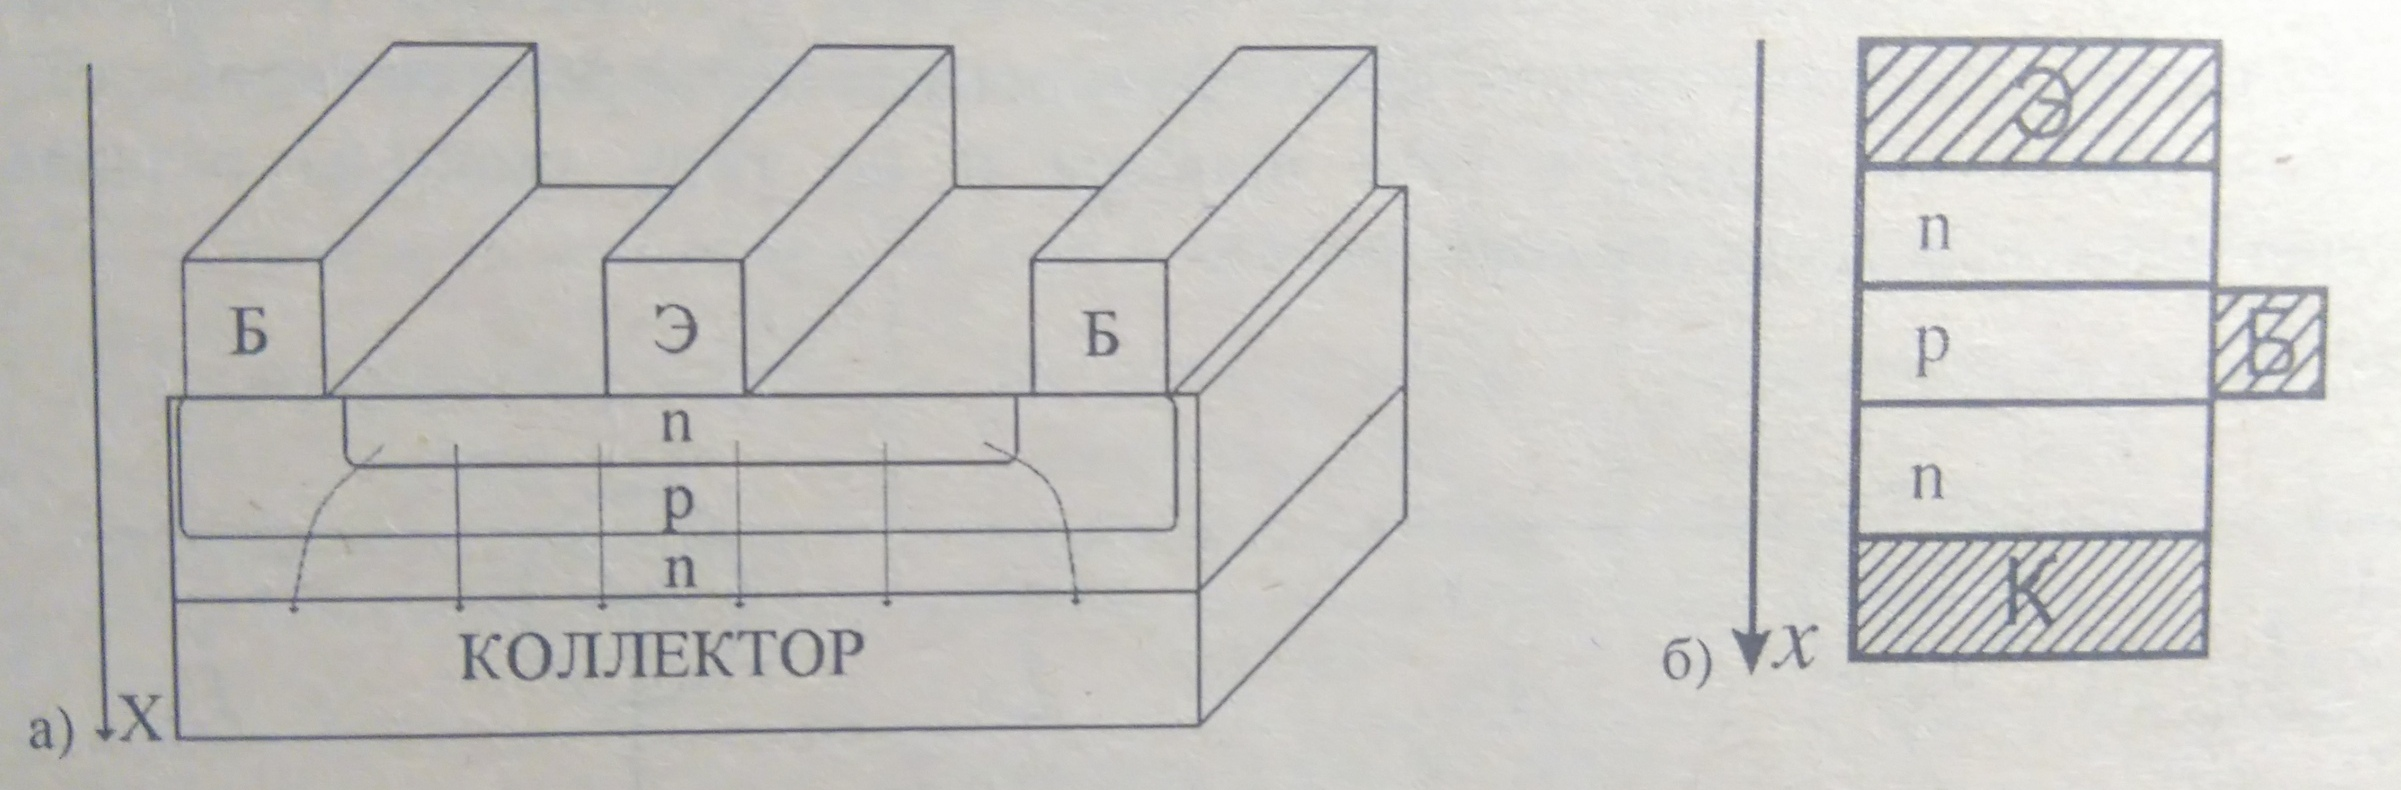
\includegraphics[width=\linewidth]{fig/1.jpg}
    \caption{}
    \label{fig:}
\end{figure}
Прибор представляет собой монокристалл, содержащий три полупроводниковых области с различным типом проводимости, которые
образуют между собой два $p-n$ перехода, а с наружными металлическими электродами -- омические контакты.

Как видно из рис. 1а ток, за исключением периферийных областей, течет перпендикулярно границам $p-n$ переходов. Обычно краевыми эффектами
на периферии структуры пренебрегают, так как толщина слоя базы много меньше её латеральных размеров. Идеализированная одномерная структура транзистора представлена на рис. 1.

Отметим две принципиальные конструктивно-технологические особенности транзисторов:
\begin{itemize}
    \item Малая толщина базы по сравнению с диффузионной длиной дырок $L_p$, являющихся в базе неосновными носителями.
    \item   Относительно малая степень легирования материла базы примесными атомами по сравнению с эмиттером и коллектора.
\end{itemize}


\subsubsection{Схема включение транзистора}%
Несмотря на то, что схема включения транзистора непосредственно не влияет на физику его работы, она определяет граничные условия на контактах.
На рис. 6 приведены две схемы включения транзистора: с общей базой (ОБ) и общим эмиттером (ОЭ).

\begin{figure}[h]
    \centering
    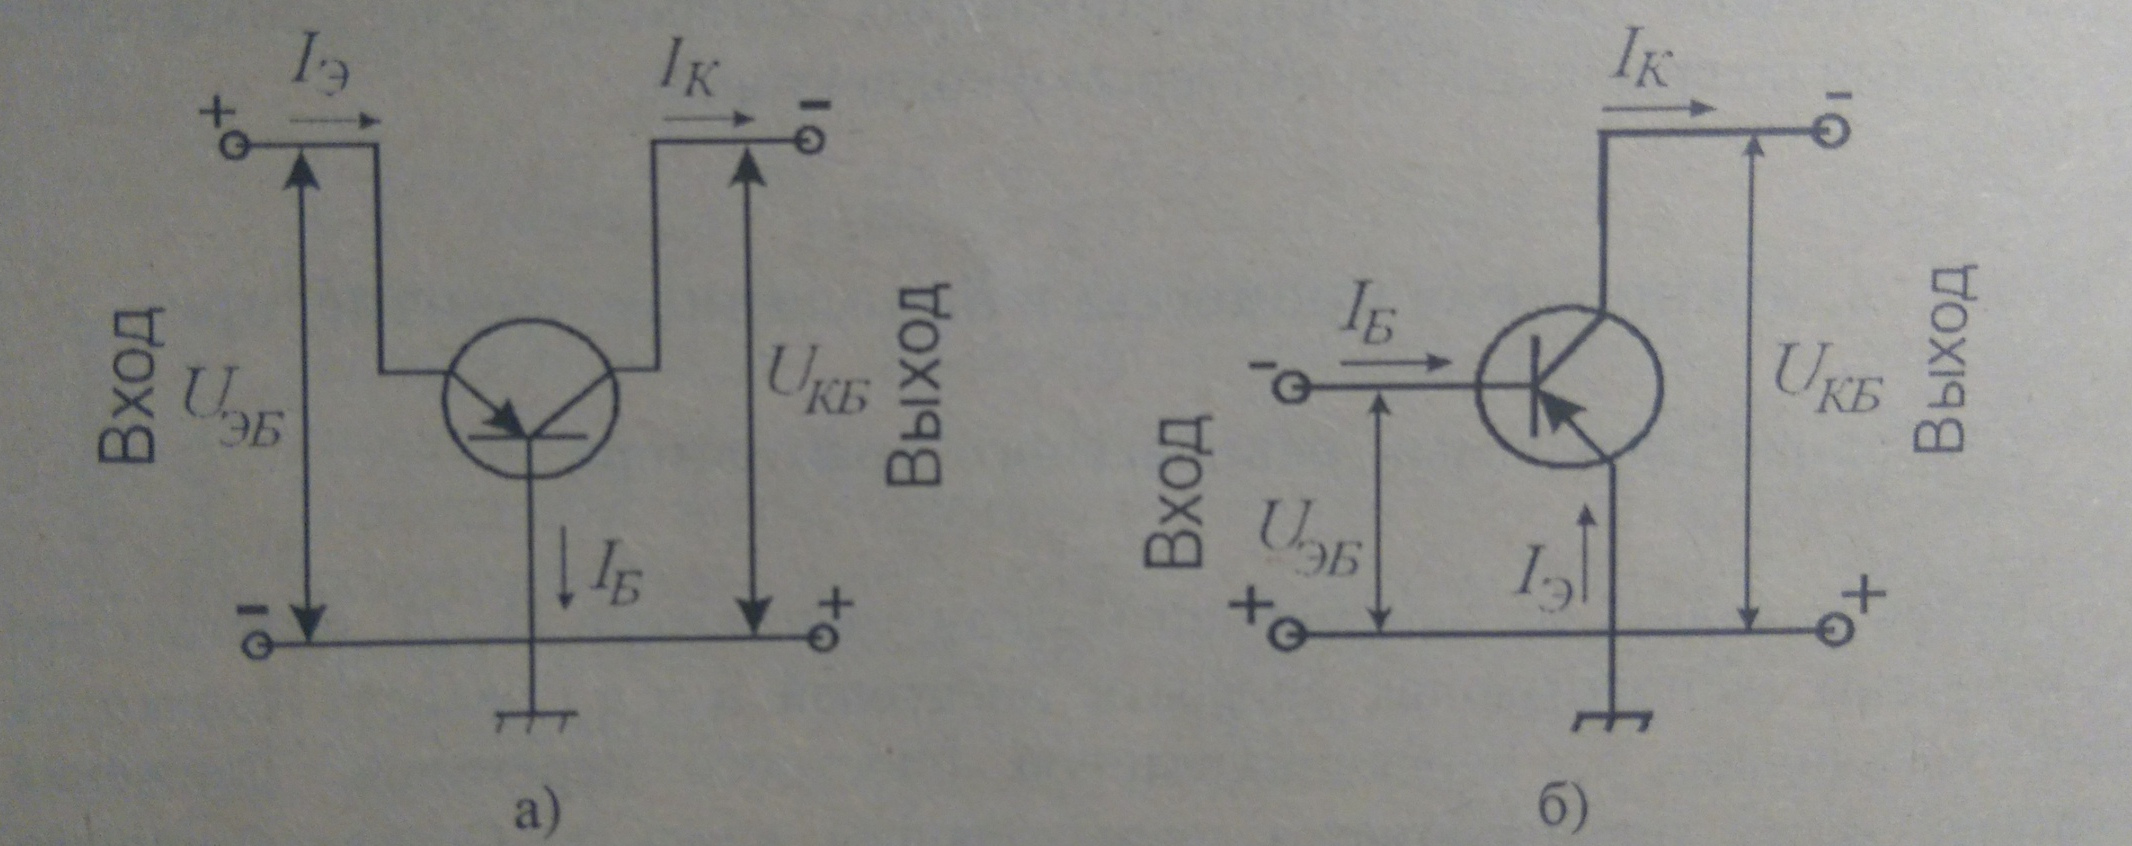
\includegraphics[width=\linewidth]{fig/2.jpg}
    \caption{}
    \label{fig:}
\end{figure}
\subsubsection{Зонная диаграмма транзистора в активном режиме}%
 Присоединим источники напряжения к клеммам транзистора. При
нормальном включении, обеспечивающим активный режим, на эмиттерный
переход должно быть подано прямое смещение, а на коллекторный переход
обратное. На рис. 2 показано включение источников по схеме с общей базой
при котором вывод базы является общим для обоих источников питания. При
малом уровне инжекции (т.е. вброса электронов и дырок соответственно
области $р$ и $n$-типа) электрическое поле вне перехода равно нулю. Тогда
на достаточном удалении от границ переходов носители находятся в состоянии
термодинамического равновесия, а уровни Ферми располагаются относительно
краев зон в соответствующих областях так же, как в равновесном транзисторе
(рис. 46). На рис. 76 изображена зонная диаграмма транзистора в активном
режиме работы.
Перепад уровней Ферми в областях $р-n$ переходов соответствие
приложенным к этим переходам напряжениям. Кроме того, приложенные
напряжения приводят к трансформации зонной диаграммы. 
\begin{itemize}
    \item Эмиттерный переход, находящийся под прямым смещением, сужается, а высота потенциального барьера в переходе уменьшается на $e_{0}U_{\text{эб}}$ ;
    \item Обратно-смещенный коллекторный переход расширяется, а высота потенциального барьера увеличивается на величину $e_0 U_{\text{кб}}$.
\end{itemize}

\begin{figure}[h]
    \centering
    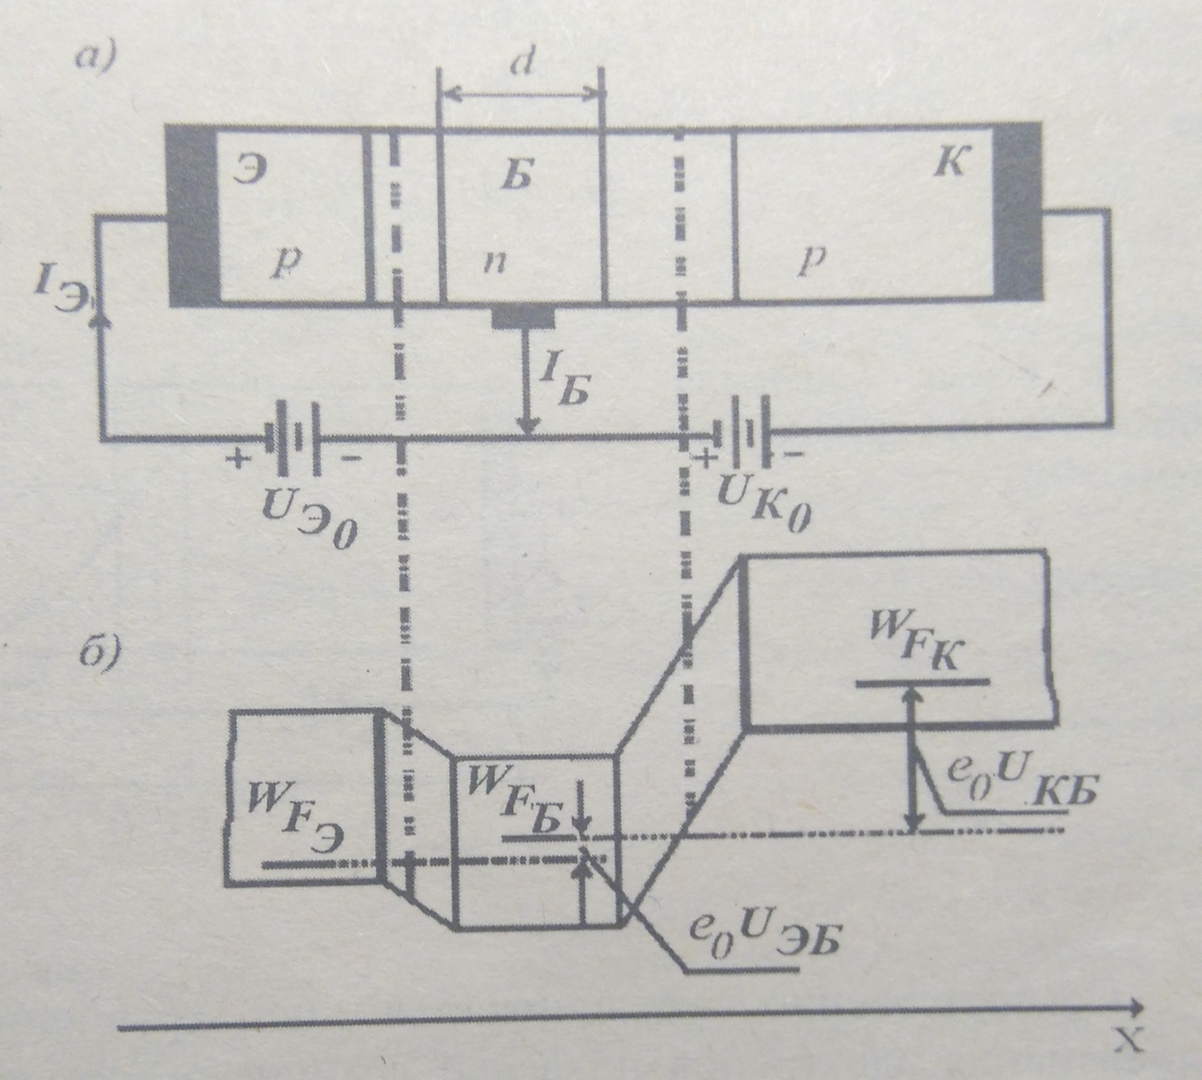
\includegraphics[width=0.5\linewidth]{fig/3.jpg}
    \caption{}
    \label{fig:}
\end{figure}
%\subsubsection{Основные процессы в транзисторе, включенном по схеме ОБ}%

%Познакомимся с принципом действия транзистора на примере схемы с ОБ. Последняя, благодаря сравнительной простоте анализа, является основной при 
%рассмотрении физических процессов.

%Подадим в эмиттерную цепь входной сигнал $U_{\text{вх}}$, а в коллекторную цепь включим  \\



\label{sec:theory}
\section{Практическая часть}%
\label{sec:practice}
\paragraph{Расчёт параметров транзистора}%
\begin{figure}[H]
    \begin{minipage}{0.49\linewidth}
        \centering
        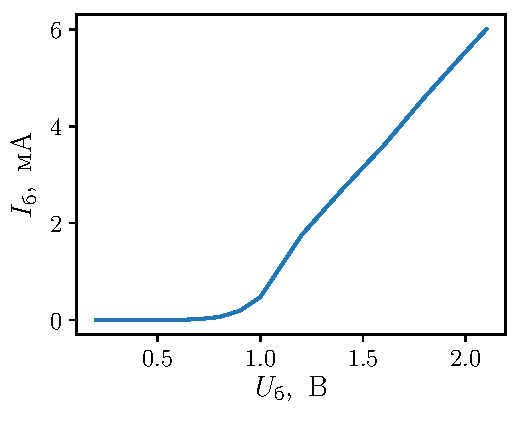
\includegraphics[scale=1]{fig/1.pdf}
        \newline
        (a)
    \end{minipage}
    \label{fig:1}
    \hfill
    \begin{minipage}{0.49\linewidth}
        \centering
        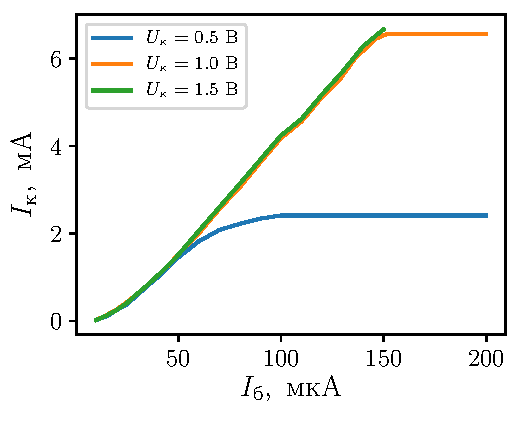
\includegraphics[scale=1]{fig/2.pdf}
        \newline
        (b)
    \end{minipage}
    \label{fig:1}
    \centering
   \begin{minipage}{0.49\linewidth}
        \centering
        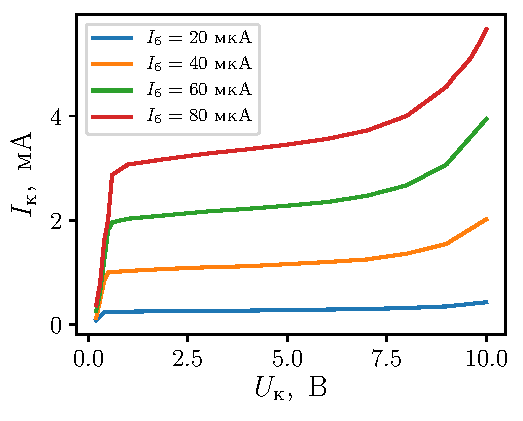
\includegraphics[scale=1]{fig/3.pdf}
        \newline
        (c)
    \end{minipage}
    \caption{Статические характеристики биполярного транзистора:
    (a) входная характеристика, (b) переходная характеристика, (c) выходная характеристика}
\end{figure}


Рассмотренные в теоретической части эквивалентные схемы не являются единственно возможными. В литературе можно встретить множество других схем, в частности, П-образные схемы.
С точки зрения схемотехники выбор конкретной схемы не имеет существенного значения. Достаточно представить транзистор в виде некоторого бесструктурного 
четырехполюсника, и задать связи между входными и выходными величинами.

В приближении малого сигнала 4-х полюсник является линейным и упомянутым связям соответствует система двух линейных уравнений.
Естественно, что коэффициенты уравнений (параметры 4-х полюсника) зависят не только от физических свойств транзистора и режима,
но также от его схемы включения и выбора каких-то двух величин из 4-х в качестве управляющих переменных.

Преимуществом такого подхода является устранение произвола, связанного с выбором той или иной эквивалентной схемы, т.к. величины
параметров определяются непосредственно из уравнений транзистора.

Рассмотрим для иллюстрации определение $h$-параметров транзистора для включения с общим эмиттером. Для
$h$-системы в качестве независимых (управляющих) переменных выбираются входной ток и выходное напряжение.
В результате уравнения линейного 4-х полюсника имеет вид:

\begin{equation}
    \begin{aligned}
        \label{eq:50}
        U_{\text{вх}} = h_{11} i_{\text{вх}} + h_{12} U_{\text{вх}},\\
        i_{\text{вых}} = h_{21} i_{\text{вх}} + h_{22} U_{\text{вых}}.
    \end{aligned}
\end{equation}
Из \eqref{eq:50} следует, что
\begin{equation}
    \begin{aligned}
        \label{eq:h}
        h_{11}= \qty( \frac{U_{\text{вх}}}{U_{\text{вых}}})\eval_{i_{\text{вх}}=0} \quad
        h_{12}= \qty( \frac{U_{\text{вх}}}{i_{\text{вх}}})\eval_{U_{\text{вых}}=0} \\
        h_{21}= \qty( \frac{i_{\text{вых}}}{i_{\text{вх}}})\eval_{U_{\text{вых}}=0} \quad
        h_{22}= \qty( \frac{i_{\text{вых}}}{U_{\text{вых}}})\eval_{i_{\text{вх}}=0}
    \end{aligned}
\end{equation}

Согласно \eqref{eq:h}, $h_{11}$ имеет смысл входного сопротивления 4-х полюсника при закороченном выходе; $h_{12}$-- коэффициент обратной связи по напряжению,
при разомкнутом входе; $h_{21}$-- коэффициент усиления по току при закороченном выходе; $h_{22}$-- выходная проводимость при разомкнутом входе.
Для системы с ОЭ:
\begin{equation}
    \label{eq:52}
    \begin{aligned}
        i_{\text{вх}}=i_{\text{б}} \quad
        i_{\text{вых}}=i_{\text{к}}\\
        U_{\text{вых}}=U_{\text{к}}+U_{\text{э}}=U_{\text{к}}^*
    \end{aligned}
\end{equation}
Отсюда можно получить $h$-параметры через основные параметры транзистора:
\begin{equation}
    \begin{aligned}
        \label{eq:53}
        &h_{11}=r_{\text{б}} + \frac{r_{\text{э}}}{1- \alpha},
        &h_{12}=\frac{r_{\text{э}}}{2(1-\alpha)r_{\text{к}}},\\
        &h_{21}=\beta=\frac{\alpha}{1-\alpha},
        &h_{22}= \frac{1}{(1-\alpha)r_{\text{к}}}
    \end{aligned}
\end{equation}

Формулы \eqref{eq:52} служат в качестве исходных при измерениях $h$-параметров. Согласно \eqref{eq:52} они определяются
из опытов при условии короткого замыкания на выходе или холостого на входе. Поскольку выходная цепь в схеме с ОЭ
является высокоомной, а входная, наоборот -- низкоомной, указанные эксперименты не вызывают затруднений. Именно
поэтому $h$-система наиболее удобна для схем с ОЭ и ОБ. Отметим, что величины $h$- одного и того же транзистора 
при различных схемах включения транзистора также различны.
По результатам проведённых измерений были рассчитаны и построены зависимости коэффициента передачи тока от напряжения коллектора при токах 
коллектора 2 мА и 5 мА. 
Для транзистора, включенного по схеме с общим эмиттером, уравнение \eqref{eq:h} примет вид
\begin{equation}
    \begin{aligned}
        \label{eq:}
       & h_{11}= \qty( \frac{U_{\text{б}}}{U_{\text{э}}})\eval_{i_{\text{к}}=0}  
       & h_{12}= \qty( \frac{U_{\text{к}}}{i_{\text{к}}})\eval_{U_{\text{э}}=0} \\
       & h_{21}= \qty( \frac{i_{\text{э}}}{i_{\text{к}}})\eval_{U_{\text{э}}=0}  \quad
       & h_{22}= \qty( \frac{i_{\text{э}}}{U_{\text{э}}})\eval_{i_{\text{к}}=0}
    \end{aligned}
\end{equation}

Коэффициент передачи по току 
\begin{equation}
    \label{eq:}
    K_{i}(U_{\text{к}}) = \frac{i_{\text{к}}}{i_{\text{б}}} = 
\end{equation}

\paragraph{Измерение коэффициента усиления однокаскадного усилителя}%
В данном опыте была собрана схема однокаскадного усилителя (см. рис. \ref{fig:7}) и произведено измерение его коэффициента 
усиления в зависимости от частоты входного сигнала.

\begin{figure}[H]
    \centering
    \includegraphics[width=0.6\linewidth]{example-image-a}
    \caption{Однокаскадный усилитель}
    \label{fig:7}
\end{figure}

\begin{figure}[H]
    \centering
    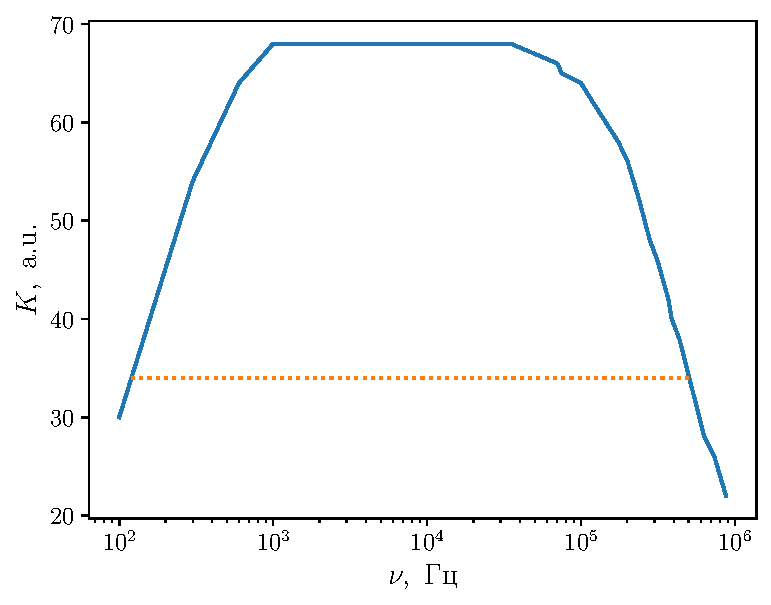
\includegraphics[scale=1]{fig/5.pdf}
    \caption{Коэффициент усиления однокаскадного усилителя. Пунктиром отмечена высота, соответствующая уровню $\frac{1}{2}$ относительно максимума}
    \label{fig:5}
\end{figure}

Полосой пропускания будем считать ординаты $K(\nu)$, соответствующие уровню 0.5 от максимума функции  $K(\nu)$.
Получаем полосу:
\begin{equation}
    \label{eq:}
         \nu_{\text{мин}} = 120 \text{ Гц}, \quad \nu_{\text{макс}} = 500 \text{ кГц} \\
\end{equation}
\begin{equation}
    \label{eq:}
     \nu_{\text{min}} < \nu < \nu_{\text{макс}} 
\end{equation}



\begin{figure}[H]
    \centering
    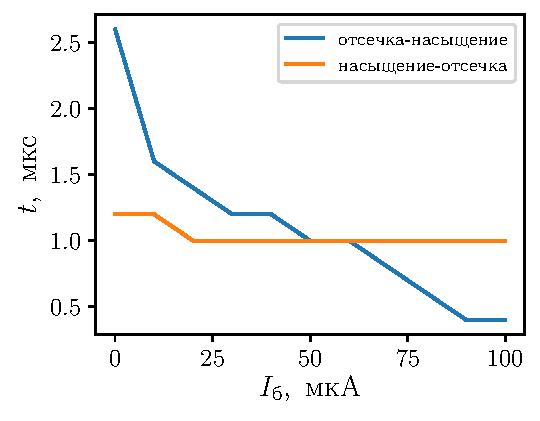
\includegraphics[scale=1]{fig/6.pdf}
    \caption{Зависимость времени переключения транзистора от тока базы транзистора}
    \label{fig:6}
\end{figure}

\end{document}
